\documentclass[a4paper, 12pt]{article}
\usepackage[utf8]{inputenc}
\usepackage[english]{babel}
\usepackage{graphicx}
\usepackage{hyperref}
\usepackage[a4paper]{geometry}
\usepackage{movie15}
\usepackage{float}
\usepackage{xcolor}
\usepackage{titlesec}
\usepackage[skins]{tcolorbox}
\usepackage[center]{caption}
%\usepackage[left=1cm,right=2cm,vmargin=2.5cm,footnotesep=0.5cm]{geometry}
\usepackage{amssymb,amsmath,amsthm}
\DeclareMathOperator*{\E}{\mathbb{E}}
\DeclareMathOperator*{\argmax}{\text{argmax}}
\DeclareMathOperator*{\Var}{\text{Var}}
\renewcommand*{\P}{\mathbb{P}}
\newtheorem{theorem}{Theorem}
\newtheorem{lemma}{Lemma}
\newtheorem{statement}{Statement}
\newtheorem{definition}{Definition}

\colorlet{sectitlecolor}{blue!40!black}
\colorlet{subsectitlecolor}{blue!40!black}
\colorlet{subsubsectitlecolor}{blue!40!black}

\titleformat{\section}
{\normalfont\Huge\bfseries\color{sectitlecolor}}{{\thesection}}{1em}{}
  
\titleformat{\subsection}
{\normalfont\Large\bfseries\color{sectitlecolor}}{{\thesection}}{1em}{}


\hypersetup{
    colorlinks=true,
    linktoc=all,
    linkcolor=[rgb]{0,0,0.35},
    filecolor=[rgb]{0,0.07,0.35},      
    urlcolor=[rgb]{0,0.07,0.35},
    bookmarks=true,
    pdfpagemode=FullScreen,
	breaklinks=true,
	bookmarksopen=false,
	pdftitle={Title},
	pdfauthor={Author}
}

  
\begin{document} 

\begin{titlepage}
	\centering
	{\scshape\LARGE Ozonmasters \par}
	\vspace{1cm}
	{\scshape\Large Statistics \par}
	\vspace{1.5cm}
	{\huge\bfseries Home work \par}
	\vspace{2cm}
	{\Large\itshape Kozhemyak Vitaly \par}
	\vfill

% Bottom of the page
	{\large \today\par}
\end{titlepage}
  
\tableofcontents

\newpage
\section*{Task 1}
\addcontentsline{toc}{section}{Task 1}
\subsection*{T1 (i)}
\addcontentsline{toc}{subsection}{T1 (i)}

\begin{tcolorbox}[enhanced,width=\textwidth,center upper,
    fontupper=\large\bfseries,drop fuzzy shadow southwest,
    colframe=red!50!black,colback=yellow!30]
\begin{statement}
Consider $X_1, \ldots, X_n$ --- i.i.d. random variables. Let $F(x)$ be a CDF of random variable $X_i, i = \{1, \ldots, n\}.$ Then 
$$
- \sum \limits_{i=1}^n \log(1 - F(X_i)) \sim \Gamma (n, 1).
$$
\end{statement}
\end{tcolorbox}

\begin{proof}
The CDF of random variable $1 - F(X_i)$ is 
$$
\P (1 - F(X_i) \leqslant x) = \P (1 - x \leqslant F(X_i)) = 1 - \P (1 - x > F(X_i)) = 1 - F(F^{-1}(1 - x)) = x.
$$
Thus, 
$$
1- F(X_i) \sim U[0, 1] \Rightarrow -\log (1 - F(X_i)) \sim Exp(1).
$$
Now we are going to use a moment-generating function $M_X(t)$ which uniquely determines a distribution. If we have $Y_1, \ldots, Y_n \sim Exp(1)$ and $S_n = Y_1 + \ldots + Y_n$ then
$$
M_{S_n}(t) = \E [e^{tS_n}] = \E [e^{t(Y_1 + \ldots + Y_n)}] = \{ i.i.d. \} = \E [e^{tY_1}] \cdot \ldots \cdot \E[e^{tY_n}] = 
$$
$$
= M_{Y_1}(t) \cdot \ldots \cdot M_{Y_n}(t) = \dfrac{1}{(1 - t)^n}, ~ t < 1.
$$
This is a moment-generating function of Gamma distribution $\Gamma(n, 1).$ If we put $Y_i = -\log (1 - F(X_i))$ we will get the statement.\\
\end{proof}
\begin{center}
\large \itshape \underline{Plotting exact confidence intervals}
\end{center}
Consider $X_1, \ldots, X_n$ --- i.i.d. random variables with Weibull CDF 
$$
F(x) = 1 - e^{-(x / \lambda)^{\tau}}, ~ x > 0.
$$
Choose the next central statistic $Z = Z(X_1,\ldots, X_n; \lambda) = \sum \limits_{i=1}^n \left( \dfrac{X_i}{\lambda} \right)^{\tau}.$
A central statistics satisfies the next rules:
\begin{enumerate}
	\item $F_Z(z)$ does not depend on $\lambda.$ Denote $Z_i = \left( \dfrac{X_i}{\lambda} \right)^{\tau}.$ Then
$$
F_{Z_i}(z) = \P (Z_i \leqslant z) = \P(X_i \leqslant \lambda x^{1/ \tau}) = 1 - e^{-x} \Rightarrow Z_i \sim Exp(1).
$$
Moreover, the result above tells us $Z = \sum \limits_{i=1}^n Z_i \sim \Gamma(n, 1).$
	\item $Z$ is continuous and strictly monotone in $\lambda.$   
\end{enumerate}
According to the definition of the exact confidence interval
$$
\P(q_{\alpha / 2} \leqslant Z \leqslant q_{1 - \alpha /2}) = 1 - \alpha,
$$
$$
\P \left( \dfrac{q_{\alpha / 2}}{\sum \limits_{i=1}^n X_i^{\tau}} \leqslant \dfrac{1}{\lambda^{\tau}} \leqslant \dfrac{q_{1 - \alpha /2}}{\sum \limits_{i=1}^n X_i^{\tau}} \right) = 1 - \alpha,
$$
\begin{tcolorbox}[enhanced,width=\textwidth,center upper,
    fontupper=\large\bfseries,drop fuzzy shadow southeast,
    colframe=red!50!black,colback=yellow!25]
$
\P \left( \left( \dfrac{q_{\alpha / 2}}{\sum \limits_{i=1}^n X_i^{\tau}} \right)^{1/ \tau} \geqslant \lambda \geqslant \left( \dfrac{q_{1 - \alpha /2}}{\sum \limits_{i=1}^n X_i^{\tau}} \right)^{1/ \tau} \right) = 1 - \alpha
$
\end{tcolorbox}
where $q_{\alpha/2}$ and $q_{1-\alpha/2}$ are left and right $\frac{\alpha}{2}$ -- quantiles of Gamma distribution $\Gamma(n, 1)$ with the significance level $\alpha$ respectively.

\subsection*{T1 (ii)}
\addcontentsline{toc}{subsection}{T1 (ii)}

Consider $X_1, \ldots, X_n \sim Exp(\lambda).$ As we know $\E [X_1] = \dfrac{1}{\lambda}, \Var [X_1] = \dfrac{1}{\lambda^2}.$
According to the CLT we have
$$
\lambda \sqrt{n} \left( \bar{X} - \dfrac{1}{\lambda} \right) \rightarrow \mathcal{N}(0, 1), ~ n \rightarrow + \infty.
$$
Consider the next two statistics 
$$
S_1(X_1, \ldots, X_n) = \dfrac{1}{n} \sum \limits_{i=1}^n X_i,
$$
$$
S_2(X_1, \ldots, X_n) = \sqrt{\dfrac{1}{2n} \sum \limits_{i=1}^n X_i^2}.
$$
\begin{center}
\large \itshape \underline{Plotting asymptotic confidence intervals using $S_1$ statistics}
\end{center}
Using the $S_1$ statistics we get
$$
\P \left( -z_{1 - \alpha/2} \leqslant \lambda \sqrt{n} \left( \bar{X} - \dfrac{1}{\lambda} \right) \leqslant z_{1- \alpha/2} \right) = 1 - \alpha,
$$
\begin{tcolorbox}
[enhanced,width=\textwidth,center upper,
 fontupper=\large\bfseries,
 drop fuzzy shadow southeast,
 colframe=red!50!black,colback=yellow!25]
$
\P \left( \dfrac{1}{\bar{X}} \left( 1 - \dfrac{z_{1 - \alpha/2}}{\sqrt{n}} \right) \leqslant \lambda \leqslant \dfrac{1}{\bar{X}} \left( 1 + \dfrac{z_{1 - \alpha/2}}{\sqrt{n}} \right) \right) = 1 - \alpha.
$
\end{tcolorbox}
The length of the confidence interval is
\begin{tcolorbox}
[enhanced,width=\textwidth,center upper,
 fontupper=\large\bfseries,
 drop fuzzy shadow southeast,
 colframe=red!50!black,colback=yellow!25]
$
l_1 = \dfrac{2}{\bar{X}} \dfrac{z_{1 - \alpha/2}}{\sqrt{n}}.
$
\end{tcolorbox}

\begin{center}
\large \itshape \underline{Plotting asymptotic confidence intervals using $S_2$ statistics}
\end{center}
Using the next formula $\left( \sigma^2 = \dfrac{1}{n} \sum \limits_{i=1}^n (X_i - \mu)^2 \right)$ we can derive the next equation 
$$
\dfrac{1}{\lambda^2} = \dfrac{1}{n} \sum \limits_{i=1}^n \left( X_i - \dfrac{1}{\lambda} \right)^2 \Rightarrow \bar{X} = \dfrac{\lambda}{2} \dfrac{1}{n} \sum \limits_{i=1}^n X_i^2.
$$	
Then
$$
\P \left( -z_{1 - \alpha/2} \leqslant \lambda \sqrt{n} \left( \bar{X} - \dfrac{1}{\lambda} \right) \leqslant z_{1- \alpha/2} \right) = 1 - \alpha,
$$
\begin{tcolorbox}
[enhanced,width=\textwidth,center upper,
 fontupper=\large\bfseries,
 drop fuzzy shadow southeast,
 colframe=red!50!black,colback=yellow!25]
$
\P \left( \sqrt{ \dfrac{2n}{\sum \limits_{i=1}^n X_i^2} \left( 1 - \dfrac{z_{1 - \alpha/2}}{\sqrt{n}} \right) } \leqslant \lambda \leqslant \sqrt{ \dfrac{2n}{\sum \limits_{i=1}^n X_i^2} \left( 1 + \dfrac{z_{1 - \alpha/2}}{\sqrt{n}} \right) } \right) = 1 - \alpha.
$
\end{tcolorbox}
The length of the confidence interval is
\begin{tcolorbox}
[enhanced,width=\textwidth,center upper,
 fontupper=\large\bfseries,
 drop fuzzy shadow southeast,
 colframe=red!50!black,colback=yellow!25]
$
l_2 = \sqrt{ \dfrac{2n}{\sum \limits_{i=1}^n X_i^2} } \cdot \left( \sqrt{ \left( 1 + \dfrac{z_{1 - \alpha/2}}{\sqrt{n}} \right) } - \sqrt{ \left( 1 - \dfrac{z_{1 - \alpha/2}}{\sqrt{n}} \right) } \right).
$
\end{tcolorbox}
Let's take a look at the plot below
\begin{figure}[H]
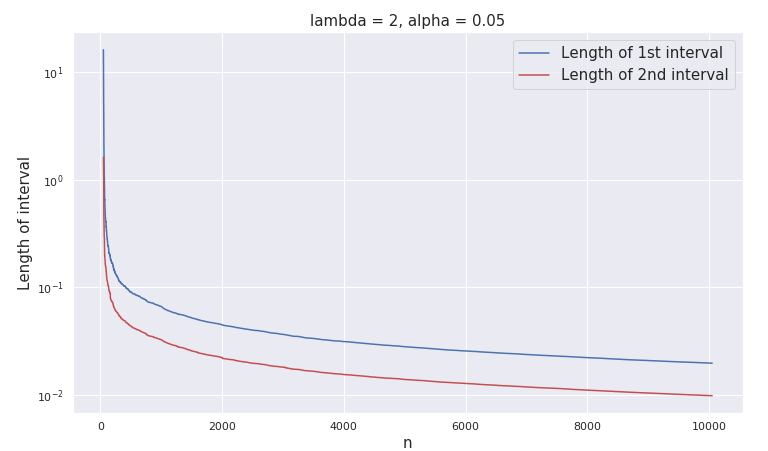
\includegraphics[width=\textwidth]{Images/1_1_2.png}
\caption{The length of the second interval is less than the length of the first interval ($l_2 < l_1$).}
\end{figure}

\subsection*{T1 (iii)}
\addcontentsline{toc}{subsection}{T1 (iii)}
Consider $X_1, \ldots, X_n$ --- i.i.d. with a CDF $F(x) = 1 - e^{-x / \lambda}.$ The order statistics $X_{(i)}, X_{(j)}, i < j$ satisfy the next equation
$$
\P \left(X_{(i)} < m = F^{-1} \left( \dfrac{1}{2} \right) < X_{(j)} \right) = \P (m < X_{(j)}) - \P (m \leqslant X_{(i)}). 
$$
Using a CDF of Binomial distribution
$$
F_{X_{(r)}}(m) = \P (X_{(r)} \leqslant m) = \sum \limits_{k=r}^n C_n^k (1 - F(m))^k (F(m))^{n-k} =$$ 
$$
= \sum \limits_{k=r}^n C_n^k \left( \dfrac{1}{2} \right)^k \left( \dfrac{1}{2} \right)^{n-k} 
= 2^{-n} \sum \limits_{k=r}^n C_n^k.
$$
Thus,
$$
\P \left(X_{(i)} < m < X_{(j)} \right) = 2^{-n} \sum \limits_{k=i}^{j-1} C_n^k.
$$
Since 
$$
F(m) = 1 - e^{-m / \lambda} = \dfrac{1}{2}
$$ 
then 
$$
m = \lambda \ln 2.
$$
Finally, 
\begin{tcolorbox}
[enhanced,width=\textwidth,center upper,
 fontupper=\large\bfseries,
 drop fuzzy shadow southeast,
 colframe=red!50!black,colback=yellow!25]
$
\P (X_{(i)} < m < X_{(j)}) = \P \left( \dfrac{X_{(i)}}{\ln 2} < \lambda < \dfrac{X_{(j)}}{\ln 2} \right) =
$
$
= 2^{-n} \sum \limits_{k=i}^{j-1} C_n^k = 1 - \alpha, ~ i < j.
$
\end{tcolorbox}


\subsection*{N1}
\addcontentsline{toc}{subsection}{N1}
\begin{figure}[H]
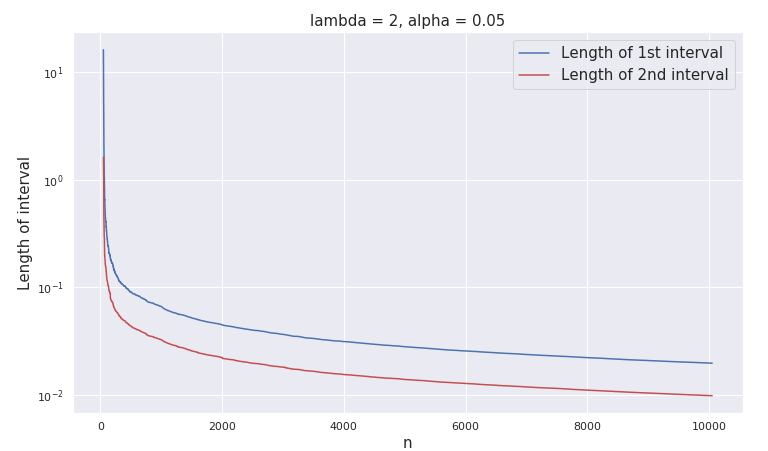
\includegraphics[width=\textwidth]{Images/1_1_2.png}
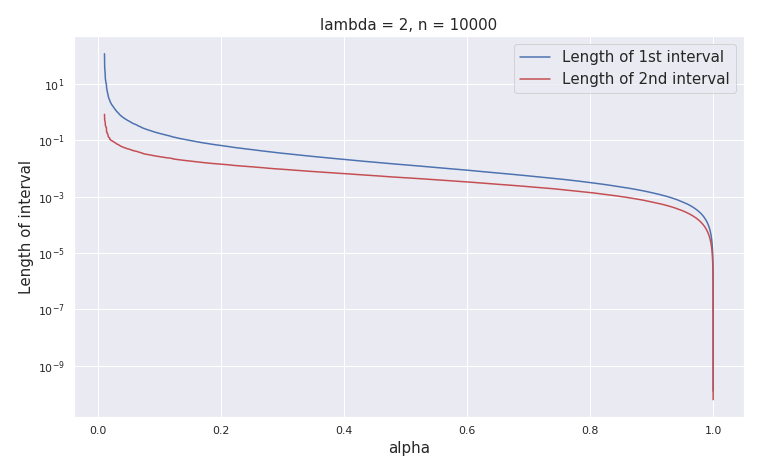
\includegraphics[width=\textwidth]{Images/1_2_1.png}
\caption{The length of the second interval is less than the length of the first interval ($l_2 < l_1$).}
\end{figure}

\section*{Task 2}
\addcontentsline{toc}{section}{Task 2}
\subsection*{T2}
\addcontentsline{toc}{subsection}{T2}
Let $X_i, Y_i$ be random variables such that
$$
X_i = 
\begin{cases}
1, & p,\\
0, & 1- p,
\end{cases}
~
Y_i = 
\begin{cases}
1, & q,\\
0, & 1- q,
\end{cases}
$$
where $p$ is probability to answer "YES" in a city, $q$ is probability to answer "YES" in a village. 
Using Central Limit Theorem we get
$$
\dfrac{\overline{X} - \overline{Y} - (p - q)}{\sqrt{\dfrac{p(1-p)}{n} + \dfrac{q(1-q)}{n}}} = \{ \text{Law of Large Numbers} \} =
$$
$$ 
= \dfrac{\overline{X} - \overline{Y} - (p - q)}{\sqrt{\dfrac{\overline{X}(1-\overline{X})}{n} + \dfrac{\overline{Y}(1-\overline{Y})}{n}}}
\rightarrow \mathcal{N}(0, 1), ~ n \rightarrow + \infty.
$$
Denote 
$$
S_n = \sqrt{\dfrac{\overline{X}(1-\overline{X})}{n} + \dfrac{\overline{Y}(1-\overline{Y})}{n}}.
$$
The confidence intervals can be calculated as following 
$$
\P \left( -z_{1-\alpha /2} \leqslant \dfrac{\overline{X} - \overline{Y} - (p - q)}{S_n} \leqslant z_{1 - \alpha /2} \right) = 1 - \alpha,
$$
$$
\P \left(\overline{X} - \overline{Y} - z_{1 - \alpha/2} S_n \leqslant p - q \leqslant \overline{X} - \overline{Y} + z_{1 - \alpha/2} S_n \right) = 1 - \alpha.
$$
We can notice that 
$$
S_n = \sqrt{\dfrac{\overline{X}(1-\overline{X})}{n} + \dfrac{\overline{Y}(1-\overline{Y})}{n}} \leqslant $$
$$
\leqslant \left \{ \overline{X} (1 - \overline{X}) \leqslant \dfrac{1}{4} \right \} \leqslant \dfrac{1}{\sqrt{2n}}.
$$
Then
$$
\P \left(\overline{X} - \overline{Y} - z_{1 - \alpha/2} \dfrac{1}{\sqrt{2n}} \leqslant p - q \leqslant \overline{X} - \overline{Y} + z_{1 - \alpha/2} \dfrac{1}{\sqrt{2n}} \right) = 1 - \alpha.
$$
Finally, $n_{min}$ is a solution of the next equation
$$
\dfrac{z_{1 - \alpha/2}}{\sqrt{2n}} = 0.05,
$$
\begin{tcolorbox}
[enhanced,width=\textwidth,center upper,
 fontupper=\large\bfseries,
 drop fuzzy shadow southeast,
 colframe=red!50!black,colback=yellow!25]
$
n_{min} = \dfrac{1}{2} \left( \dfrac{z_{1 - \alpha/2}}{0.05} \right)^2, ~ \alpha = 0.05.
$
\end{tcolorbox}

\subsection*{T3}
\addcontentsline{toc}{subsection}{T3}
Consider a null hypothesis $H_0: p - q = 0$ and an alternative $H_1: p - q = 0.03.$ Let's calculate the Test Statistics
$$
T = \dfrac{\overline{X} - \overline{Y} - (p - q)}{\sqrt{\dfrac{p(1-p)}{n} + \dfrac{q(1-q)}{n}}} = \dfrac{\overline{X} - \overline{Y} - (p - q)}{\sqrt{\dfrac{\overline{X}(1-\overline{X})}{n} + \dfrac{\overline{Y}(1-\overline{Y})}{n}}} = \sqrt{n} \dfrac{0.05 - (p-q)}{\sqrt{0.2023}}.
$$
Reject the null hypothesis if 
$$
T > z_{1-\alpha}
$$ 
where $z_{1-\alpha}$ is a $1-\alpha$-quantile of $\mathcal{N}(0, 1).$ \\
Let's calculate type 1 error as following
$$
\P(\text{error 1 type}) = \P (\text{reject }H_0 \, | \, H_0 \text{ is true}) = \P(T > z_{1-\alpha} | p = q).
$$
Let's calculate type 2 error as following
$$
\P(\text{error 2 type}) = \P (\text{don't reject }H_0 \, | \, H_0 \text{ is false}) = \P(T \leqslant z_{1-\alpha} | p = q + 0.03).
$$
Since we want that
$$
\P(\text{error 1 type}) = 0.05,
$$
$$
\P(\text{error 2 type}) = 0.04,
$$
we have to solve the next system of inequalities
$$
\begin{cases}
\sqrt{n} \dfrac{0.05}{\sqrt{0.2023}} > z_{0.95} = 1.65, \\
\sqrt{n} \dfrac{0.02}{\sqrt{0.2023}} \leqslant z_{0.96} = 1.76, \\
\end{cases}
\Leftrightarrow
\begin{cases}
n > 250.65, \\
n < 1566.61. \\
\end{cases}
$$
Finally, we get
\begin{tcolorbox}
[enhanced,width=\textwidth,center upper,
 fontupper=\large\bfseries,
 drop fuzzy shadow southeast,
 colframe=red!50!black,colback=yellow!25]
$
n_{min} = 251.
$
\end{tcolorbox}

\section*{Task 3}
\addcontentsline{toc}{section}{Task 3}
\subsection*{T4}
\addcontentsline{toc}{subsection}{T4}
Consider a null hypothesis $H_0: \theta = \theta_0,$ an alternative $H_1: \theta > \theta_0$ and
\begin{tcolorbox}
[enhanced,width=\textwidth,center upper,
 fontupper=\large\bfseries,
 drop fuzzy shadow southeast,
 colframe=red!50!black,colback=yellow!25]
\textbf{\small LR (Likelihood Ratio) test}
$$
\lambda(\vec{x}) = \dfrac{\mathcal{L}(\vec{x}, \theta_0)}{\sup \limits_{\theta \geqslant \theta_0} \mathcal{L}(\vec{x}, \theta)}.
$$
\end{tcolorbox}
Let $\hat{\theta}$ be the solution for the next problems $\sup \limits_{\theta \geqslant \theta_0} \mathcal{L}(\vec{x}, \theta).$ Now the LR can be written as following
$$
\lambda(\vec{x}) = \left( \dfrac{\theta_0}{\hat{\theta}} \right)^n \prod \limits_{i=1}^n (1-x_i)^{\theta_0- \hat{\theta}}.
$$
Thus, we accept $H_0$ if 
$$
\lambda(\vec{x}) \geqslant c \Leftrightarrow n \log \left(\dfrac{\theta_0}{\hat{\theta}} \right) + (\theta_0 - \hat{\theta}) \sum \limits_{i=1}^n \log (1 - x_i) \geqslant \log c. 
$$
Denote $$
\widetilde{c} = \dfrac{ \log c - n \log \left(\dfrac{\theta_0}{\hat{\theta}} \right)}{\theta_0 - \hat{\theta}}.
$$
\begin{center}
\large \itshape \underline{Searching for the threshold $c$}
\end{center}
To find the constant $\widetilde{c}$ we are going to calculate a type 1 error
$$ 
\P(\text{type 1 error}) = \P (\text{reject } H_0| H_0 \text{ is true}) = \P \left( \sum \limits_{i=1}^n \log (1 - x_i) < \widetilde{c} \, | \, H_0 \text{ is true} \right).
$$
\begin{tcolorbox}
[enhanced,width=\textwidth,center upper,
 fontupper=\large\bfseries,
 drop fuzzy shadow southeast,
 colframe=red!50!black,colback=yellow!25]
\begin{statement}
Consider $X_1, \ldots, X_n \sim p(x;\theta).$ Then
$$
\sum \limits_{i=1}^n \log (1 - X_i) \sim \Gamma \left( n, \dfrac{1}{\theta} \right).
$$
\end{statement}
\end{tcolorbox}
\begin{proof}
Consider exponential random variable $X \sim p(x; \theta).$ Then
$$
F_{\log(1-X)}(x) = \P (\log(1 - X) \leqslant x) = 1 - F_X(1 - e^x).
$$
Recall that
$$
F_X(x) = 
\begin{cases}
0, & x < 0, \\
1 - (1 - x)^{\theta}, & 0 \leqslant x \leqslant 1, \\
1, & x > 1.
\end{cases}
$$
Thus, we have
$$
F_{\log(1-X)}(x) = e^{x \theta} \Leftrightarrow f_{\log(1-X)}(x) = \theta e^{x \theta} \sim Exp(\theta), ~ x \in ( -\infty, 0].
$$
As we know 
$$
\sum \limits_{i=1}^n \log (1 - X_i) \sim \Gamma \left( n, \dfrac{1}{\theta} \right).
$$
\end{proof}
\noindent Back to the type 1 error
$$ 
\P(\text{type 1 error}) = \P \left( \sum \limits_{i=1}^n \log (1 - x_i) < \widetilde{c} \, | \, H_0 \text{ is true} \right) = F_{(n, \theta_0)}(\widetilde{c}) = \alpha,
$$
$$
\widetilde{c} = F_{(n, \theta_0)}^{-1}(\alpha) = q_{(n, \theta_0)}(\alpha)$$
Threshold $c$ can be found the next way
\begin{tcolorbox}
[enhanced,width=\textwidth,center upper,
 fontupper=\large\bfseries,
 drop fuzzy shadow southeast,
 colframe=red!50!black,colback=yellow!25]
$
c = \exp \left( (\theta_0 - \hat{\theta}) \cdot q_{(n, \theta_0)}(\alpha) + n \log \left( \dfrac{\theta_0}{\hat{\theta}} \right) \right)
$
\end{tcolorbox}
where $F_{(n, \theta_0)}$ is a CDF of Gamma distribution $\Gamma \left( n, \dfrac{1}{\theta_0} \right),$ and $q_{(n, \theta_0)}(\alpha)$ is a $\alpha$ -- quantile of Gamma distribution $\Gamma \left( n, \dfrac{1}{\theta_0} \right)$ (if we consider the left tailed test).\\

\begin{center}
\large \itshape \underline{The power of test}
\end{center}
According to the definition of the power of statistic test
$$
W(\theta) = \P (\text{reject } H_0 \, | \, H_1 \text{ is true}) = 
$$
$$
= \P \left( \sum \limits_{i=1}^n \log (1 - x_i) < \widetilde{c} \, | \, H_1 \text{ is true} \right) = F_{(n, \theta)}(q_{(n, \theta_0)}(\alpha)),
$$
where $F_{(n, \theta)}$ is a CDF of Gamma distribution $\Gamma \left( n, \dfrac{1}{\theta} \right)$ and $\theta > \theta_0.$
Finally, we have
$$
W(\theta) = F_{(n, \theta)}(q_{(n, \theta_0)}(\alpha)) = \int \limits_{0}^{q_{(n, \theta_0)}(\alpha)} \dfrac{\theta^n t^{n-1} e^{-t \theta}}{ \Gamma(n)} dt = 
$$
$$
= \left \{ z = \dfrac{\theta}{\theta_0} t \right \} = \dfrac{\theta_0}{\theta} \int \limits_{0}^{\dfrac{\theta}{\theta_0} \cdot q_{(n, \theta_0)}(\alpha)} \dfrac{\theta^n \theta_0^{n-1}}{\theta^{n-1}} \dfrac{z^{n-1} e^{-t \theta_0}}{\Gamma(n)} dz = F_{(n, \theta_0)} \left( \dfrac{\theta}{\theta_0} \cdot q_{(n, \theta_0)} \right).
$$
\begin{tcolorbox}
[enhanced,width=\textwidth,center upper,
 fontupper=\large\bfseries,
 drop fuzzy shadow southeast,
 colframe=red!50!black,colback=yellow!25]
$
W(\theta) = F_{(n, \theta_0)} \left( \dfrac{\theta}{\theta_0} \cdot q_{(n, \theta_0)} \right).
$
\end{tcolorbox}

\subsection*{T5}
\addcontentsline{toc}{subsection}{T5}
Note that 
\begin{tcolorbox}
[enhanced,width=\textwidth,center upper,
 fontupper=\large\bfseries,
 drop fuzzy shadow southeast,
 colframe=red!50!black,colback=yellow!25]
$\bar{X} \sim \mathcal{N} \left( \mu, \dfrac{\sigma^2}{n} \right).$
\end{tcolorbox}
Let 
$$
E_1(c) = \P(\bar{X} > c | \mu = \mu_0) = 1- \P(\bar{X} \leqslant c | \mu = \mu_0) = 1- \int \limits_{-\infty}^{c} \dfrac{\sqrt{n}}{\sqrt{2 \pi \sigma^2}} e^{-\dfrac{n (x-\mu_0)^2}{2 \sigma^2}} dx
$$
be a type 1 error and 
$$
E_2(c) = \P(\bar{X} \leqslant c | \mu = \mu_1) = \int \limits_{-\infty}^{c} \dfrac{\sqrt{n}}{\sqrt{2 \pi \sigma^2}} e^{-\dfrac{n (x-\mu_1)^2}{2 \sigma^2}} dx
$$
be a type 2 error.\\
Using the optimality condition we get
$$
\dfrac{d (E_1(c) + E_2(c))}{dc} = 0,
$$ 
$$
 \dfrac{\sqrt{n}}{\sqrt{2 \pi \sigma^2}} e^{-\dfrac{n (c-\mu_1)^2}{2 \sigma^2}} =  \dfrac{\sqrt{n}}{\sqrt{2 \pi \sigma^2}} e^{-\dfrac{n (c-\mu_0)^2}{2 \sigma^2}},
$$
\begin{tcolorbox}
[enhanced,width=\textwidth,center upper,
 fontupper=\large\bfseries,
 drop fuzzy shadow southeast,
 colframe=red!50!black,colback=yellow!25]
$
c = \dfrac{\mu_1 + \mu_0}{2}.
$
\end{tcolorbox}

\section*{Task 4}
\addcontentsline{toc}{section}{Task 4}
\subsection*{T6* (i)}
\addcontentsline{toc}{subsection}{T6* (i)}
Let's denote
\begin{tcolorbox}
[enhanced,width=\textwidth,center upper,
 fontupper=\large\bfseries,
 drop fuzzy shadow southeast,
 colframe=red!50!black,colback=yellow!25]
$
\hat{\theta} = \argmax \limits_{\theta \geqslant \theta_0} \mathcal{L}(\vec{x}, \theta) = \argmax \limits_{\theta \geqslant \theta_0} \prod \limits_{i=1}^n p(x_i, \theta).
$
\end{tcolorbox}
Then 
\begin{equation}
\label{lab1}
\Lambda(\vec{x}) = \dfrac{\mathcal{L}(\vec{x}, \hat{\theta})}{\mathcal{L}(\vec{x}, \theta_0)} \geqslant 0
\end{equation}
be a likelihood ratio.
Consider the log-likelihood ratio, normalized dividing by $n:$
$$
\Lambda_n(\vec{x}) = \dfrac{1}{n} \log \dfrac{\mathcal{L}(\vec{x}, \hat{\theta})}{\mathcal{L}(\vec{x}, \theta_0)} = \dfrac{1}{n} \sum \limits_{i=1}^n \log \dfrac{p(x_i, \hat{\theta})}{p(x_i, \theta_0)}.
$$
Note $X_1, \ldots, X_n$ are i.i.d. and $L_i = \log \dfrac{p(x_i, \hat{\theta})}{p(x_i, \theta_0)}$ is a random variable. In addition, we know from the strong Law of Large Numbers that
$$
\dfrac{1}{n} \sum \limits_{i=1}^n \log \dfrac{p(x_i, \hat{\theta})}{p(x_i, \theta_0)} \rightarrow \E [L_1], ~ n \rightarrow +\infty.
$$ 
By definition of expected value
$$ 
\E [L_1] = \int \limits_{-\infty}^{+\infty} q(x) \log \dfrac{p(x, \hat{\theta})}{p(x, \theta_0)} dx \geqslant 0
$$
where we can put $q(x) = p(x, \theta_0)$ and then
\begin{tcolorbox}
[enhanced,width=\textwidth,center upper,
 fontupper=\large\bfseries,
 drop fuzzy shadow southeast,
 colframe=red!50!black,colback=yellow!25]
$
\E [L_1] = \int \limits_{-\infty}^{+\infty} p(x, \theta_0) \log \dfrac{p(x, \hat{\theta})}{p(x, \theta_0)} dx = K(\theta_0, \hat{\theta}).
$
\end{tcolorbox}
Finally, 
\begin{tcolorbox}
[enhanced,width=\textwidth,center upper,
 fontupper=\large\bfseries,
 drop fuzzy shadow southeast,
 colframe=red!50!black,colback=yellow!25]
$
\log \Lambda(\vec{x}) = n \E [L_1] = 
\begin{cases}
n K(\theta_0, \hat{\theta}) & \hat{\theta} > \theta_0 \\
0, & \hat{\theta} = \theta_0.
\end{cases}
$
\end{tcolorbox}
\subsection*{T6* (ii)}
\addcontentsline{toc}{subsection}{T6* (ii)}
Using \eqref{lab1} we can rewrite LR test as following
$$
\mathcal{L}(\vec{x}, \hat{\theta}) \geqslant c_{\alpha} \mathcal{L}(\vec{x}, \theta_0),
$$
$$
\prod \limits_{i=1}^n e^{x_i \hat{\theta} - d(\hat{\theta})} \geqslant c_{\alpha} \prod \limits_{i=1}^n e^{x_i \theta_0 - d(\theta_0)},
$$
$$
\sum \limits_{i=1}^n (x_i \hat{\theta} - d(\hat{\theta})) \geqslant \log c_{\alpha} + \sum \limits_{i=1}^n (x_i \theta_0 - d(\theta_0)),
$$
$$
\hat{\theta} \geqslant \theta_0 + \dfrac{\log c_{\alpha} + n d(\hat{\theta}) - n d(\theta_0)}{\sum \limits_{i=1}^n x_i}.
$$
If we denote $\widetilde{c}_{\alpha} = \dfrac{\log c_{\alpha} + n d(\hat{\theta}) - n d(\theta_0)}{\sum \limits_{i=1}^n x_i}$ then
\begin{tcolorbox}
[enhanced,width=\textwidth,center upper,
 fontupper=\large\bfseries,
 drop fuzzy shadow southeast,
 colframe=red!50!black,colback=yellow!25]
$
\hat{\theta} \geqslant \theta_0 + \widetilde{c}_{\alpha}.
$
\end{tcolorbox}

\section*{Appendix}
\addcontentsline{toc}{section}{Appendix}
\begin{itemize}
	\item Source code can be found \href{https://github.com/vitomania/ozon/blob/master/stats/hw3/hw3.ipynb}{here}.
\end{itemize}

\end{document} 